¿Cuál es el \'area del paralelogramo de la figura \ref{fig:area_compuesta_04}?

\begin{figure}[H]
    \begin{center}
        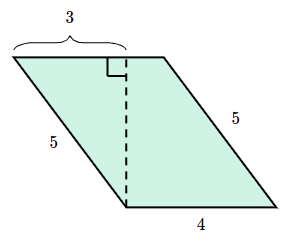
\includegraphics[width=0.3\linewidth]{../images/area_compuesta_04.png}
    \end{center}
    \caption{}
    \label{fig:area_compuesta_04}
\end{figure}
\begin{solutionbox}{15cm}

    \begin{minipage}{0.6\textwidth}
        Para determinar el área del paralelogramo debemos saber la base y la altura. Llamemos $x$ a la altura (ver Figura \ref{fig:area_compuesta_04a}).
        Cuando tenemos un triángulo rectángulo, podemos usar el teorema de Pitágoras para obtener la longitud del cateto.
        La ecuación para el teorema de Pitágoras es:
        \[c^2=a^2+b^2\]
        En este caso, $a=3$, $b=x$ y $c=5$, Entonces,
        \begin{align*}
            3^2+x^2 & =5^2  \\
            9+x^2   & =25   \\
            x^2     & =25-9 \\
            x^2     & =16   \\
            x       & =4
        \end{align*}
        La base del paralelogramo es 4 y la altura 4. El área del paralelogramo es:

        \begin{align*}
            A & =bx             \\
            A & =4\cdot 4       \\
            A & =16 \text{ u}^2
        \end{align*}
    \end{minipage}\hfill
    \begin{minipage}{0.35\textwidth}
        \begin{figure}[H]
            \centering
            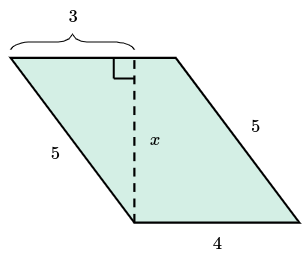
\includegraphics[width=0.9\linewidth]{../images/area_compuesta_04a.png}
            \caption{}
            \label{fig:area_compuesta_04a}
        \end{figure}
    \end{minipage}

\end{solutionbox}
